\documentclass[12pt,a4paper]{article}

\usepackage[T1,T2A]{fontenc}
\usepackage[utf8]{inputenc}
\usepackage[english, russian]{babel}
\usepackage{indentfirst}
\usepackage{misccorr}
\usepackage{graphicx}
\usepackage{amsmath}
\usepackage{graphicx}
\usepackage{float}
\usepackage[left=20mm,right=10mm, top=20mm,bottom=20mm,bindingoffset=0mm]{geometry}

\setlength{\parskip}{6pt}
\DeclareGraphicsExtensions{.png}

\begin{document}

    \begin{titlepage}
        \begin{center}
            \large
            Санкт-Петербургский политехнический университет\\Петра Великого\\
            \vspace{0.5cm}
            Институт прикладной математики и механики\\
            \vspace{0.25cm}
            Кафедра «Прикладная математика»
            \vfill
            \textsc{\LARGE\textbf{Курсовая работа}}\\[5mm]
            \Large
            по дисциплине\\"Математическая статистика"\\по теме: "Калибровка шкалы измерителя"
        \end{center}
        \vfill
        \begin{tabular}{l p{175} l}
            Выполнила студентка\\группы 3630102/80201 && Деркаченко Анна Олеговна
            \vspace{0.25cm}
            \\Проверил\\доцент, к.ф.-м.н. && Баженов Александр Николаевич
        \end{tabular}
        \vfill
        \begin{center}
            Санкт-Петербург\\2021 г.
        \end{center}
    \end{titlepage}

\newpage
\begin{center}
    \tableofcontents
    \setcounter{page}{2}
\end{center}
\newpage
\begin{center}
    \listoffigures
\end{center}

\newpage
\section{Постановка задачи}
Дано множество данных, снятых с измерителя. Требуется откалибровать шкалу измерителя с помощью имеющихся данных. Для этого небходимо:
\begin{enumerate}
    \item Определить амплитуду гармонического сигнала по набору отсчетов
    \item Определить фазы отсчетов по амплитуде
    \item Использовать интервальный подход к решению переопределенных СЛАУ для точного определения амплитуды
\end{enumerate}

\section{Теория}
\subsection{Интервальный анализ}
\textbf{Опр: \textit{интервал}} - замкнутый отрезок вещественной оси ($A=[a,b]$).

\textbf{Опр: \textit{интервальная неопределенность}} - состояние неполного знания об интересующейся величине. В таком случае возможно указать лишь границы допустимых значений данной величины, причем величина принимает все значения из интервала с равной долей вероятности.

\begin{center}
    \textbf{\textit{Алгебра интервалов:}}
\end{center}
\begin{itemize}
    \item $\overline{A}+\underline{A}=[\overline{a},\overline{b}]+[\underline{a},\underline{b}]=[\overline{a}+\underline{a},\overline{b}+\underline{b}]$
    \item $\overline{A}-\underline{A}=[\overline{a},\overline{b}]-[\underline{a},\underline{b}]=[\overline{a}-\underline{a},\overline{b}-\underline{b}]$
    \item $\overline{A}*\underline{A}=[\overline{a},\overline{b}]*[\underline{a},\underline{b}]=[min(\overline{a}\underline{a},\overline{a}\underline{b},\overline{b}\underline{a},\overline{b}\underline{b}),max(\overline{a}\underline{a},\overline{a}\underline{b},\overline{b}\underline{a},\overline{b}\underline{b})]$
    \item $\frac{\overline{A}}{\underline{A}}=\frac{[\overline{a},\overline{b}]}{[\underline{a},\underline{b}]}=[\overline{a},\overline{b}]*[\frac{1}{\underline{a}},\frac{1}{\underline{b}}]$
\end{itemize}

\textbf{Опр: \textit{интервальная матрица}} - матрица вида:
\begin{equation}
    A=
        \begin{pmatrix}
            a_{11} & ... & a_{1n}\\
            ... & ... & ...\\
            a_{m1} & ... & a_{mn}\\
        \end{pmatrix}
\end{equation}
где $a_{ij}$ - интервал, $i=\overline{1,m},j=\overline{1,n}$.

\textbf{Опр: \textit{интервальная система линейных алгебраических уравнений (ИСЛАУ):}}
\begin{equation}
    \left\{
    \begin{array}{ll}
        a_{11}x_1+...+a_{1n}x_n=b_1\\
        ...\\
        a_{m1}x_1+...+a_{mn}x_n=b_m\\
    \end{array}
    \right.
\end{equation}
где $a_{ij},b_i$ - интервалы, $i=\overline{1,m},j=\overline{1,n}$, или $Ax=B$, где $A=(a_{ij})$ - интервальная матрица, $B=(b_i)$ - интервальный вектор.

\textbf{\textit{Множество решений ИСЛАУ:}}
\begin{itemize}
    \item Объединенное множество $\Theta_{uni}(A,B)=\{x\in{\mathbf{R}^n}|\exists{A'}\in{A},\exists{B'}\in{B},A'x=B'\}$
    \item Допусковое множество $\Theta_{tol}(A,B)=\{x\in{\mathbf{R}^n}|\forall{A'}\in{A},\exists{B'}\in{B},A'x=B'\}$
\end{itemize}
При этом $\Theta_{tol}(A,B)\subseteq{\Theta_{uni}(A,B)}$.

Допусковое множество решений может оказаться пустым, если интервалы правой части слишком узки в сравнении с интервалами элементов матрицы.

\subsubsection{Задача восстановления зависимости}
Пусть $A$ - интервальная матрица, $B$ - интервальный столбец эмпирических данных. Тогда $Ax=B$ - ИСЛАУ, где $x_1,...,x_n$ - оценки исходных параметров.

Решение данного ИСЛАУ в общем случае представляет собой множество $\Theta_{uni}(A,B)$. Если требуется сильное согласование параметров с интервальными экспериментальными данными, то решением является множество $\Theta_{tol}(A,B)$.

\subsubsection{Метод максимального согласования}
\textbf{Теорема:} точка $x\in{\mathbf{R}^n}$ принадлежит допусковому множеству решений ИСЛАУ $\Theta_{tol}(A,B)\Longleftrightarrow{Ax\subseteq{B}}$.

\textbf{Опр: \textit{распознающий функционал}} - $Tol(x,A,B)=min_{1\leq{i}\leq{m}}{rad(b_i)}-|\sum_{j=1}^na_{ij}x_j-mid(b_i)|$, где $rad(a)=\frac{1}{2}(\overline{a}-\underline{a}),mid(a)=\frac{1}{2}(\overline{a}+\underline{a})$ для интервала $a$.

Тогда $\Theta_{tol}(A,B)=\{x\in{\mathbf{R}^n}|Tol(x,A,B)\geq0\}$.

В качестве оценки параметров берется точка, в которой достигается наибольшее неотрицательное значение данного распознающего функционала.

\section{Ход работы}
При получении сигналов с измерителя может наблюдаться нерегулярность отсчетов и амплитудная неточность (сдвиг амплитуд). При этом для сигналов с частотой выше нескольких десятков мегагерц необходимо использовать форму гармонических сигналов, чтобы достичь точности в $10\%$. Частота сигналов при этом очень стабильна, а амплитуда считается неизвестной, так как при дискретизации сигналов данные имеют бинарный формат, не связанный с установками прибора, генерирующего сигнал.

Таким образом, решение задачи разбивается на этапы:
\begin{enumerate}
    \item Амплитудная калибровка
        \begin{enumerate}
            \item Подать поочередно сигналы констант и построить по ним усредненные значения для каждой ячейки (набор уровней)
            \item Построить кусочно-линейную интерполяцию сигнала 
        \end{enumerate}
    \item Интервальный анализ временной калибровки
        \begin{enumerate}
            \item Определить параметры гармонического сигнала по амплитудным значениям
            \item Определить фазы отсчетов сигнала
        \end{enumerate}
\end{enumerate}

\subsection{Определение параметров гармонического сигнала}
Необходимо выполнить масштабирование исходной выборки $\{y_i\}$ - амплитудные значения сигнала в промежуток $[0,1]$ и вычислить амплитуду арксинуса как пересечение прямых, проходящих через линейно зависимые точки. При этом учитываем, что амплитудные значения $y_i$ даны с погрешностью.

\textbf{\textit{Алгоритм поиска коэффициентов прямой $y=a^+x+b^+$ с положительным наклоном:}}
\begin{enumerate}
    \item Найти множество точек $I^+=\{I^+_{k0},...,I^+_{kn}\}$, где $I^+_{ki}$ - множество точек, лежащих на одной прямой с положительным наклоном
    \item При этом каждая точка должна удовлетворять условию $y=a^+i+b^++dk$, где $d$ - смещение из-за периода
    \item Построить интервальные оценки по спецификации прибора для $i:[i-\frac{1}{2},i+\frac{1}{2}]$, для $y:[y-0.015|y|,y+0.015|y|]$
    \item Составить ИСЛАУ, подставив соответствующие интервальные оценки в СЛАУ вида:
        \begin{equation}
            \begin{pmatrix}
                i_0 & 1 & 0\\
                ... & ... & ...\\
                i_j & 1 & k\\
                ... & ... & ...\\
                i_n & 1 & l\\        
            \end{pmatrix}
            \begin{pmatrix}
                a\\
                b\\
                d\\
            \end{pmatrix}
            =
            \begin{pmatrix}
                y_0\\
                ...\\
                y_j\\
                ...\\
                y_n\\        
            \end{pmatrix}
        \end{equation}
        где $i_j\in{I^+_{kj}}$
    \item Применить метод максимального согласования для нахождения оценок параметров $a$ и $b$
\end{enumerate}

Таким образом, с помощью найденных $a^+,b^+,a^-,b^-$ находится амплитуда арксинуса как ордината точки пересечения соответствующих прямых.

\subsection{Определение фаз отсчетов сигнала}
Необходимо провести масштабирование $\{y_i\}$ так, чтобы амплитуда стала равной $\frac{\pi}{2}$. Тогда $\Delta{t_i}=\frac{\Delta{y_i}}{2\pi\nu}$. При этом временной интервал вычисляется для точек, по котором производилось построение прямых, а временной интервал между соседними измерениями $\Delta{t_i}$ вычисляется как среднее по всем сигналам.

\section{Реализация}
Реализация курсовой работы проводилась на языке Python в среде разработки PyCharm c использованием дополнительных библиотек:
\begin{itemize}
    \item numpy
    \item matplotlib
    \item math
    \item seaborn
    \item tolsolvty
\end{itemize}

Исходный код лабораторной работы размещен в GitHub-репозитории:

URL: https://github.com/derkanw/Mathstat/tree/main/coursework

\section{Результаты}
\begin{figure}[H]
    \centering
    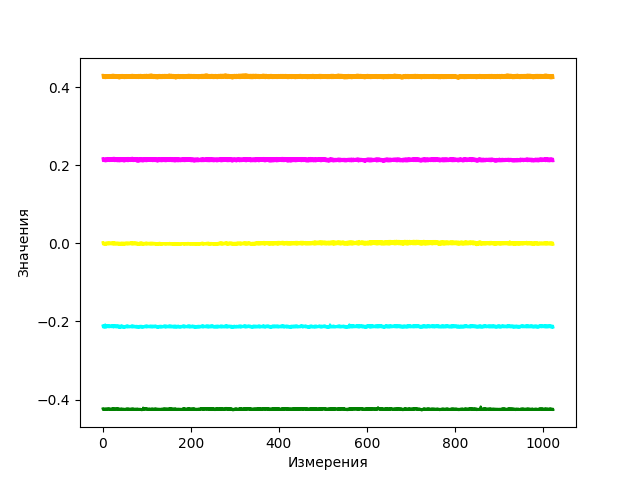
\includegraphics[scale=0.8]{images/levels.png}
    \caption{Амплитуды входного сигнала при измерении константных сигналов, цветом обозначены разные значения констант}
\end{figure}

\begin{figure}[H]
    \centering
    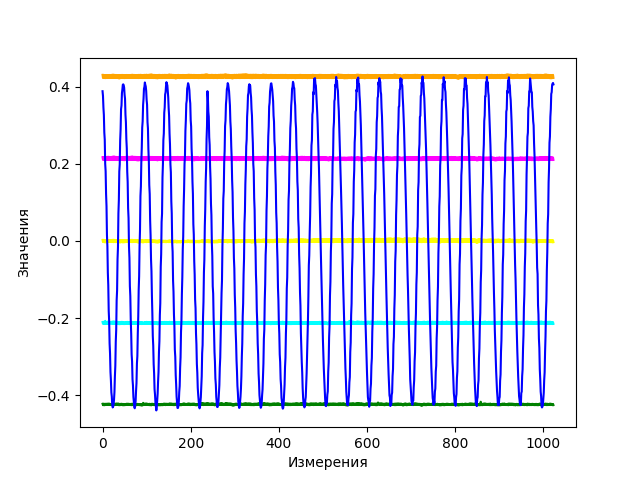
\includegraphics[scale=0.8]{images/signal_in_levels.png}
    \caption{Оцифрованный сигнал с иллюстрацией константных сигналов}
\end{figure}

\begin{figure}[H]
    \centering
    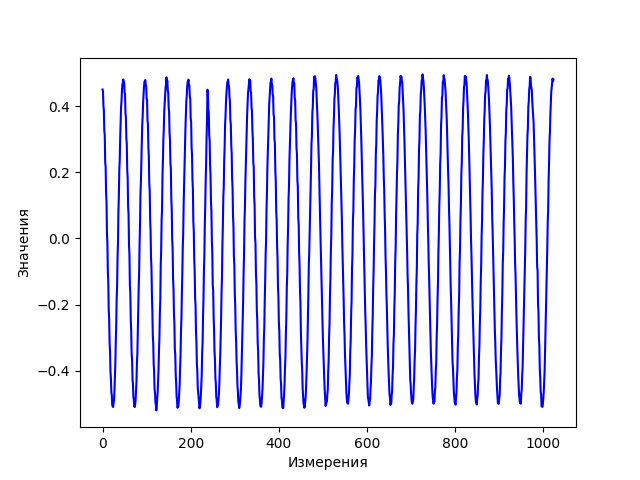
\includegraphics[scale=0.8]{images/interpolation.png}
    \caption{Интерполированный сигнал}
\end{figure}

\begin{figure}[H]
    \centering
    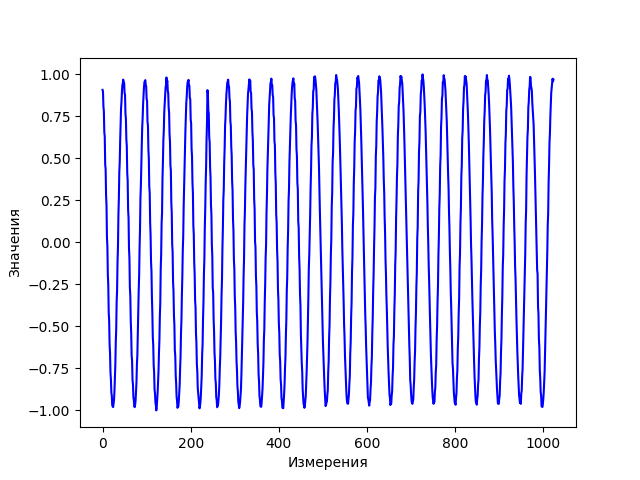
\includegraphics[scale=0.8]{images/one_scale.png}
    \caption{Масштабированный сигнал на [0,1]}
\end{figure}

\begin{figure}[H]
    \centering
    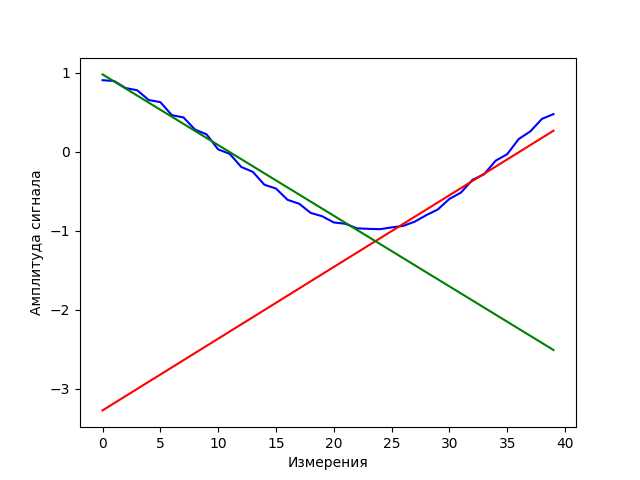
\includegraphics[scale=0.8]{images/amlitude.png}
    \caption{Нахождение амплитуды сигнала}
\end{figure}

\begin{figure}[H]
    \centering
    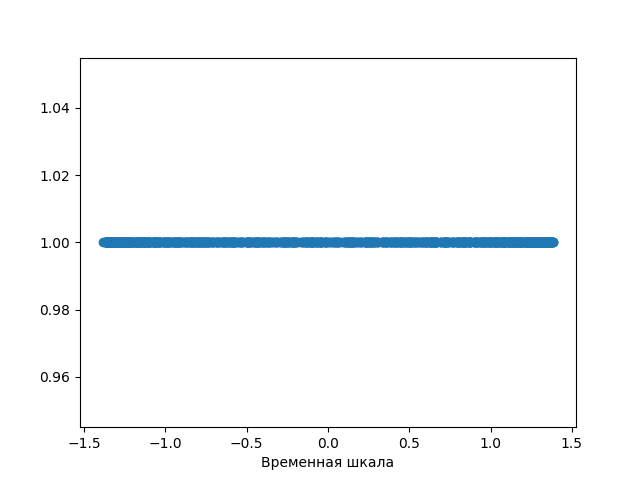
\includegraphics[scale=0.8]{images/time.png}
    \caption{Временная шкала сигнала}
\end{figure}

\begin{figure}[H]
    \centering
    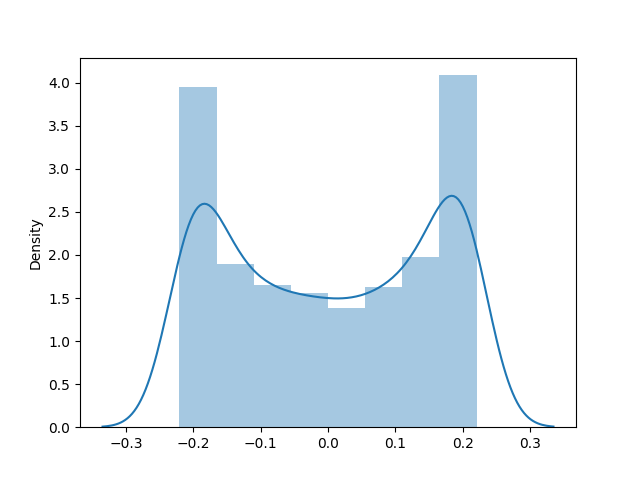
\includegraphics[scale=0.8]{images/hist.png}
    \caption{Гистограмма распределения ширин временных бинов}
\end{figure}

\section{Обсуждение}
Графики исходного сигнала и сигнала после интерполяции схожи. Это свидетельствует о том, что исходные данные о сигнале заданы по закону, который хорошо просматривается и имеет достаточную гладкость.

Для получения временной шкалы были использованы почти все точки сигнала, что является особенностью реализованного метода. При этом используется форма гармонических сигналов, что позволяет обрабатывать сигналы с частотой выше нескольких десятков мегагерц с достаточной точностью (порядка 10\%).

Для нахождения амплитуды сигнала используется функция арксинуса, которая нивелирует проблему недостаточности точек, так как позволяет использовать почти все точки, а не только в линейной области гармонической функции вблизи нуля.

Амплитуда арксинуса ищется как пересечение прямых, проходящих через
линейно зависимые точки. При этом касательные к ним не являются симметричными, что объясняется неточностью генерации сигнала.

Использование интервального анализа для поиска коэффициента прямых позволяет учитывать погрешности данных в виде неравномерных временных отсчетов и погрешности амплитудных значений.

На гистограмме распределения временных ширин наблюдается бимодальность, что соответствует заявленному распределению в работе [1].

\section{Список используемой литературы}
\begin{thebibliography}{1}
\bibitem{VKR}
Билев Ф.А. Исследование применения интервального подхода к задаче калибровки шкалы измерителя с нерегулярными отсчетами // Бакалаврская работа. / Рук.: Баженов А.Н. - С.-П. : СПБПУ. - 2017. - 31 с.
\end{thebibliography}
\end{document}
